\input{header}

\AtBeginSubsection[]
{
	\begin{frame}<beamer>
		\frametitle{Outline}
		\tableofcontents[current,currentsubsection]
	\end{frame}
}

\begin{document}
\begin{frame}[allowframebreaks] \frametitle{Computability theory vs. complexity theory}
    \begin{itemize}
\item In Chapter 3 we showed that various TMs are equivalent
\item For example, single-tape and multi-tape TMs are equivalent
\item However, their ``time complexity'' are different
\end{itemize}\end{frame}

\begin{frame}[allowframebreaks] \frametitle{Complexity of Multi-tape
  TM}
  \begin{itemize}
  \item Theorem 7.8
    
  \item [] $O(t(n))$ multi-tape TM

$\Rightarrow \exists$ equivalent 
$O(t(n)^2)$ single-tape TM
\item Idea for the proof: similar to how we proved their equivalence

\item Show that simulating each step of a multi-tape TM
takes
$O(t(n))$ on a single-tape TM

\item Let $k$ be the number of tapes
\item How did we simulate a multi-tape TM?

\begin{center}
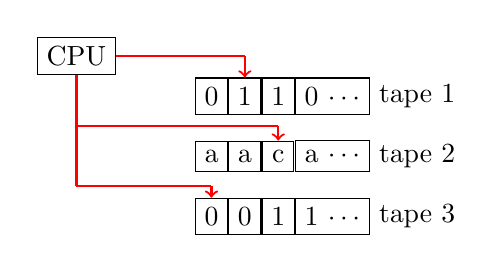
\begin{tikzpicture}[ampersand replacement=\&]
\matrix 
{
  \node[draw](0) {CPU}; \& [1cm]  \& \node(1){} ; \&\&\& \\
  \& \node[draw]{0}; \& \node[draw](a){1}; \& \node[draw]{1}; \& \node[draw]{0 $\cdots$};  \& \node{tape 1};\\
\node(2){} ; \&  \&  \& \node(21){} ; \&\& \\  
\& \node[draw]{a}; \& \node[draw]{a}; \& \node[draw](b){c}; \& \node[draw]{a $\cdots$}; \&  \node{tape 2}; \\
\node(3){} ; \& \node(31){} ; \&  \&  \&\& \\
\& \node[draw](c){0}; \& \node[draw]{0}; \& \node[draw]{1}; \& \node[draw]{1 $\cdots$}; \&  \node{tape 3}; \\
};

\draw [-,red,thick] (0) -- (1.center) ;
\draw [->,red,thick] (1.center) -- (a) ;
\draw [-,red,thick] (0) -- (2.center) ;
\draw [-,red,thick] (2.center) -- (21.center) ;
\draw [->,red,thick] (21.center) -- (b) ;
\draw [-,red,thick] (0) -- (3.center) ;
\draw [-,red,thick] (3.center) -- (31.center) ;
\draw [->,red,thick] (31.center) -- (c) ;
\end{tikzpicture}
\end{center}


\begin{center}
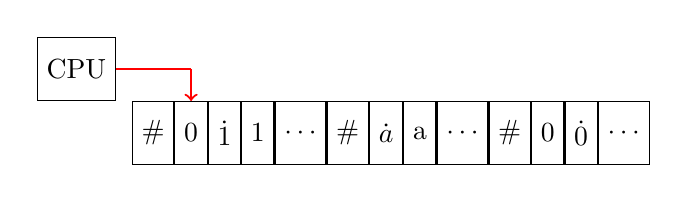
\begin{tikzpicture}[ampersand replacement=\&]
\matrix[nodes={minimum height=8mm}] 
{
  \node[draw](0) {CPU}; \& [0.2cm] \& \node(1){} ; \&\& \&\&\& \&\&\& \&\&\& \\
\& \node[draw]{\#};  \& \node[draw](a){0}; \& \node[draw]{$\dot{1}$}; \& \node[draw]{1}; \& \node[draw]{$\cdots$};
\& \node[draw]{\#};  \& \node[draw]{$\dot{\text{a}}$}; \& \node[draw]{a}; \& \node[draw]{$\cdots$}; 
\& \node[draw]{\#};  \& \node[draw](c){0}; \& \node[draw]{$\dot{0}$}; \& \node[draw]{$\cdots$}; \\
};

\draw [-,red,thick] (0) -- (1.center) ;
\draw [->,red,thick] (1.center) -- (a) ;
\end{tikzpicture}
\end{center}

\item Simulate each step of multi-tape TM: scan to know where heads point to
  and do the update
\item However, we may have to
right shift the tape 
\item So we need to know the tape length. It is
\begin{equation*}
  k \times O(t(n)) = O(t(n)) 
\end{equation*}
\item Why $O(t(n))$?
  
\item Each tape of multi-tape TM has $O(t(n))$ length

\item [] An $O(t(n))$ multi-tape TM generates
$O(t(n))$ contents in 
$O(t(n))$ time (note that $O(t(n))\geq n$).

\item Thus the cost of
  simulating each step of multi-tape TM on a single-tape TM is
  $O(t(n))$
\item There are $O(t(n))$ multi-tape TM steps, so
  the total cost is
  \begin{equation*}
    O(t(n)) \times O(t(n)) = O(t(n)^2)
\end{equation*}
\end{itemize}\end{frame}

\begin{frame}[allowframebreaks] \frametitle{Complexity of Nondeterministic TM}
  \begin{itemize}
\item Remember NTM a decider if all branches halt on all inputs

\item Definition of NTM time complexity $f(n)$:

\item [] maximum \# of steps the machine uses on any branch
on any input length $n$

\item Theorem 7.11
\item [] For an $t(n) \geq n, O(t(n))$ NTM (single tape)

\item [] $\Rightarrow \exists \text{ a } 2^{O(t(n))}$ TM (single tape)
\item Assume $b$ is the maximal number of branches at each layer
\item Recall that we use a depth-first way for the simulation
\item Total number of nodes in the tree:
  \begin{equation*}
  O(b^{t(n)})
\end{equation*}
\item Depth $d$ finished, do $d+1$

\item Tape 3: all possible paths so far

\item Tape 2: original input w, simulate one path, 1 step further
with all possible branches


\item Cost of running from root to one node in tape 2: $O(t(n))$

\item Update of tape 3: $O(b^{(t(n))})$

\item Total cost $\leq O(b^{t(n)})$ for each node
\item Total time:

  \begin{equation*}
    \begin{split}
& \# \text{ nodes } \times \text{ cost per node}\\      
= &   O(b^{t(n)}) \times O(b^{t(n)}) \\
= & O((b^2)^{t(n)} ) = O(2^{t(n)})
\end{split}
\end{equation*}

\item This is by a 3-tape TM
\item To use a single-tape TM to simular a 3-tape one, we need
  \begin{equation*}
(2^{O(t(n))})^2
= 2^{O(t(n))}
\end{equation*}
cost because
\begin{equation*}
  (2^{O(t(n))})^2
\leq (2^{ct(n)})^2
= 2^{2ct(n)} 
= 2^{O(t(n))}
\end{equation*}
\end{itemize}\end{frame}

\end{document}
